\documentclass{beamer}
\usetheme{Madrid}

\title[Automatic Night Lamp]{Automatic Night Lamp\\with BC547 Transistor LED Night Light LDR}
\author[hashir khan]{hashir khan ,muhammad shahbaz, waqas atta}
\date{\today}

\begin{document}

\begin{frame}
  \titlepage
\end{frame}

\section{Introduction}
\begin{frame}{Introduction}
  \frametitle{Introduction}
  \begin{itemize}
    \item Good morning/afternoon/evening, ladies and gentlemen.
    \item Today, I am delighted to present an innovative project titled \textit{Automatic Night Lamp with BC547 Transistor LED Night Light LDR}.
    \item Aims to design an intelligent and energy-efficient night lamp.
    \item Automatically turns on in darkness and turns off during daylight.
    \item Utilizes a Light Dependent Resistor (LDR) and a BC547 transistor.
  \end{itemize}
\end{frame}

\section{Components}
\begin{frame}{Components}
  \frametitle{Components}
  \begin{itemize}
    \item Small LDR (Light Dependent Resistor)
    \item BC547 Transistor
    \item 3V LED (Light Emitting Diode)
    \item 1k Resistor
    \item 10k Resistor
  \end{itemize}
\end{frame}

\section{Advantages}
\begin{frame}{Advantages}
  \frametitle{Advantages}
  \begin{itemize}
    \item Energy Efficiency
    \item Convenience
    \item Cost-Effectiveness
    \item Customizability
  \end{itemize}
\end{frame}

\section{Disadvantages}
\begin{frame}{Disadvantages}
  \frametitle{Disadvantages}
  \begin{itemize}
    \item Limited Range
    \item Dependency on Ambient Light
  \end{itemize}
\end{frame}

\section{Circuit Diagram}
\begin{frame}{Circuit Diagram}
  \frametitle{Circuit Diagram}
  \begin{figure}[htbp]
    \centering
    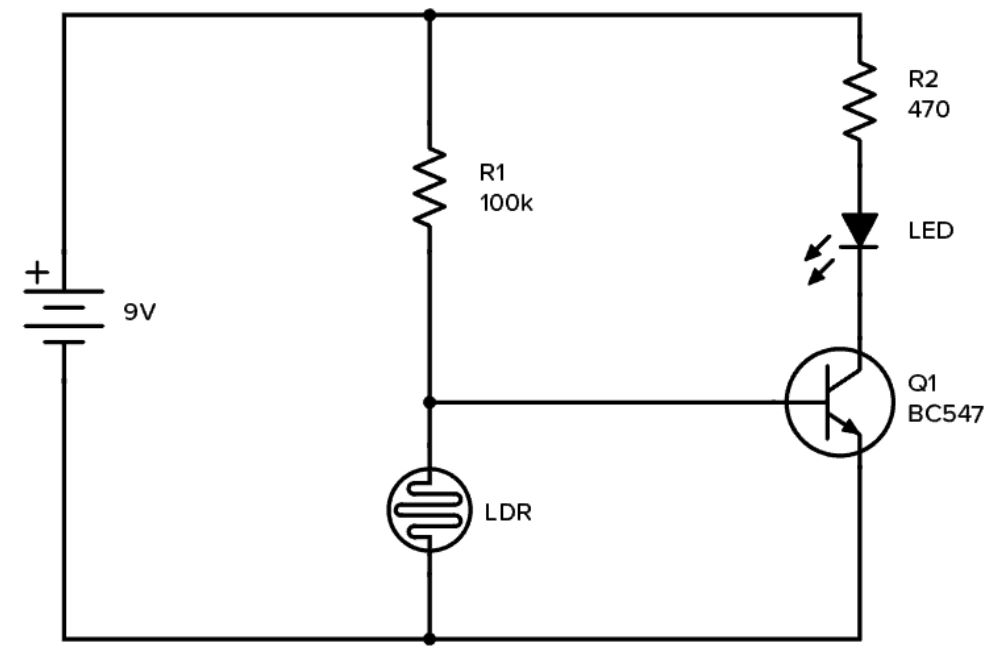
\includegraphics[width=0.8\textwidth]{1.png}
    \caption{Circuit diagram of the Automatic Night Lamp with BC547 Transistor LED Night Light LDR project.}
  \end{figure}
\end{frame}

\section{Conclusion}
\begin{frame}{Conclusion}
  \frametitle{Conclusion}
  \begin{itemize}
    \item The \textit{Automatic Night Lamp with BC547 Transistor LED Night Light LDR} project provides an intelligent and energy-efficient solution for nighttime illumination.
    \item Incorporates a small LDR, BC547 transistor, LED, and appropriate resistors.
    \item Automatically turns on in darkness and turns off during daylight hours.
    \item Simplicity, cost-effectiveness, and customizability make it a valuable addition to modern lighting systems.
  \end{itemize}
\end{frame}

\end{document}
